\documentclass{standalone}

\usepackage{tikz}

\begin{document}
    


\tikzset{every picture/.style={line width=0.75pt}} %set default line width to 0.75pt        

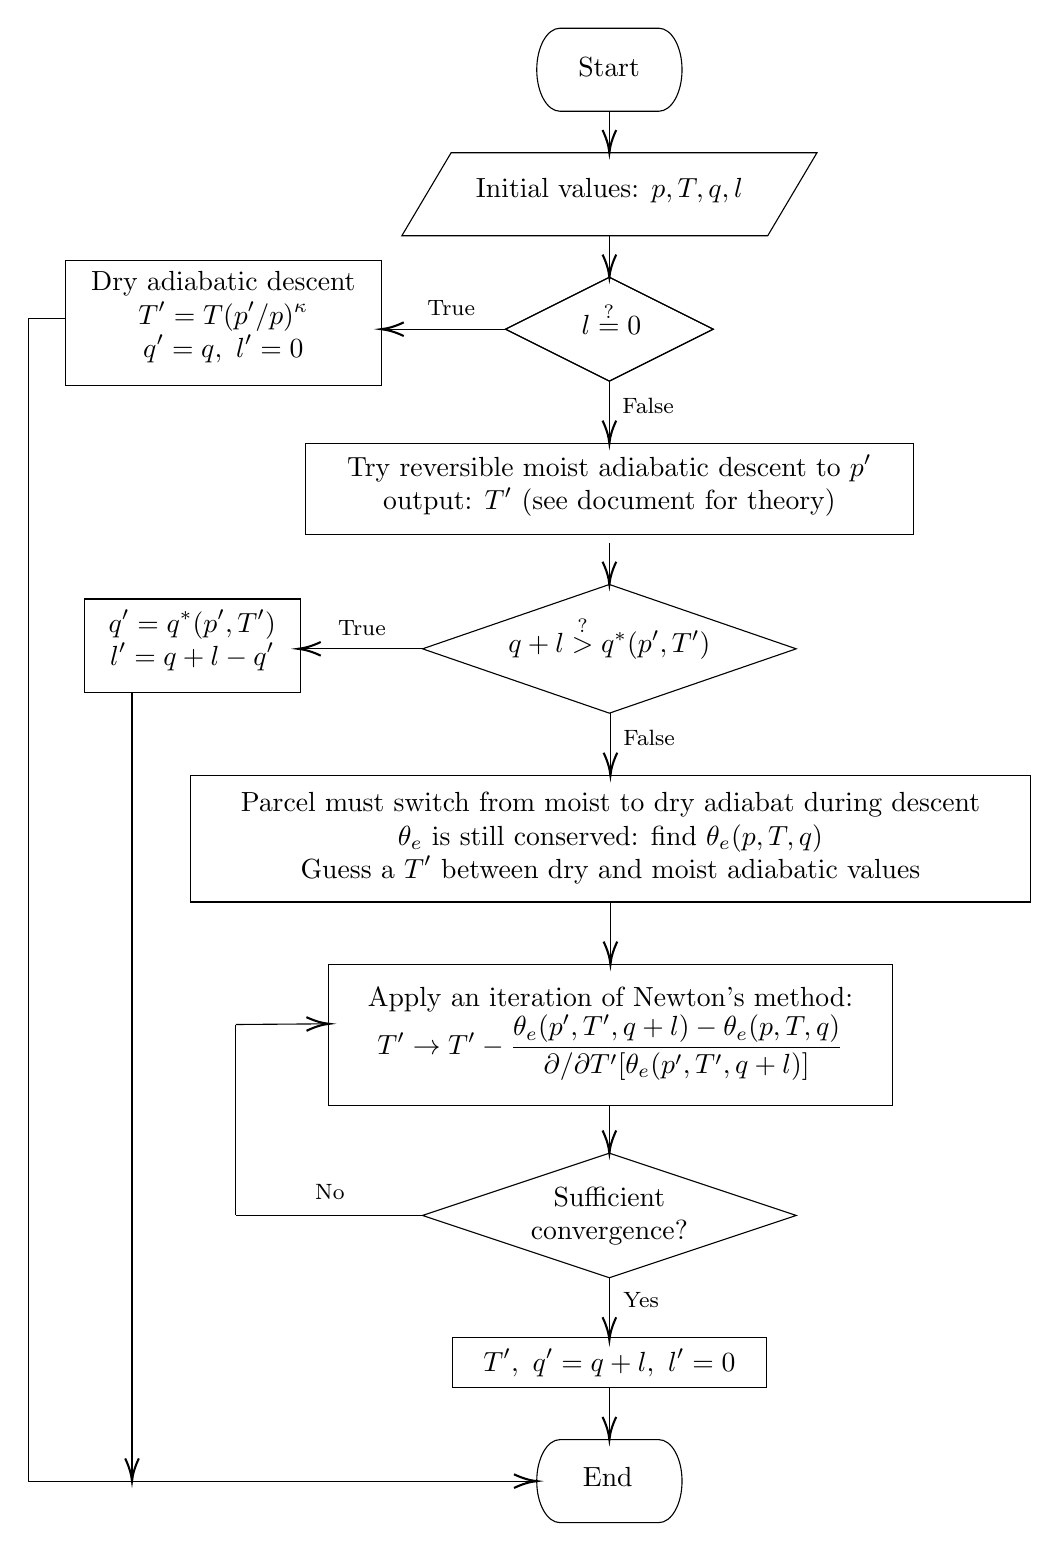
\begin{tikzpicture}[x=0.75pt,y=0.75pt,yscale=-1,xscale=1]
%uncomment if require: \path (0,864); %set diagram left start at 0, and has height of 864

%Flowchart: Terminator [id:dp8976510592531053] 
\draw   (296.2,60) -- (343.8,60) .. controls (349.99,60) and (355,68.95) .. (355,80) .. controls (355,91.05) and (349.99,100) .. (343.8,100) -- (296.2,100) .. controls (290.01,100) and (285,91.05) .. (285,80) .. controls (285,68.95) and (290.01,60) .. (296.2,60) -- cycle ;
%Shape: Parallelogram [id:dp28777739701110394] 
\draw   (243.73,120) -- (420,120) -- (396.27,160) -- (220,160) -- cycle ;
%Straight Lines [id:da9476630445843837] 
\draw    (320,100) -- (320,118) ;
\draw [shift={(320,120)}, rotate = 270] [color={rgb, 255:red, 0; green, 0; blue, 0 }  ][line width=0.75]    (10.93,-3.29) .. controls (6.95,-1.4) and (3.31,-0.3) .. (0,0) .. controls (3.31,0.3) and (6.95,1.4) .. (10.93,3.29)   ;
%Flowchart: Decision [id:dp7940368948840619] 
\draw   (320,180) -- (370,205) -- (320,230) -- (270,205) -- cycle ;
%Straight Lines [id:da24064437976531838] 
\draw    (320,160) -- (320,178) ;
\draw [shift={(320,180)}, rotate = 270] [color={rgb, 255:red, 0; green, 0; blue, 0 }  ][line width=0.75]    (10.93,-3.29) .. controls (6.95,-1.4) and (3.31,-0.3) .. (0,0) .. controls (3.31,0.3) and (6.95,1.4) .. (10.93,3.29)   ;
%Straight Lines [id:da4714326866707328] 
\draw    (270,205) -- (212,205) ;
\draw [shift={(210,205)}, rotate = 360] [color={rgb, 255:red, 0; green, 0; blue, 0 }  ][line width=0.75]    (10.93,-3.29) .. controls (6.95,-1.4) and (3.31,-0.3) .. (0,0) .. controls (3.31,0.3) and (6.95,1.4) .. (10.93,3.29)   ;
%Straight Lines [id:da8386533033760315] 
\draw    (320,230) -- (320,258) ;
\draw [shift={(320,260)}, rotate = 270] [color={rgb, 255:red, 0; green, 0; blue, 0 }  ][line width=0.75]    (10.93,-3.29) .. controls (6.95,-1.4) and (3.31,-0.3) .. (0,0) .. controls (3.31,0.3) and (6.95,1.4) .. (10.93,3.29)   ;
%Flowchart: Decision [id:dp4110956009277027] 
\draw   (320,180) -- (370,205) -- (320,230) -- (270,205) -- cycle ;
%Straight Lines [id:da9806083154690015] 
\draw    (320,308) -- (320,326) ;
\draw [shift={(320,328)}, rotate = 270] [color={rgb, 255:red, 0; green, 0; blue, 0 }  ][line width=0.75]    (10.93,-3.29) .. controls (6.95,-1.4) and (3.31,-0.3) .. (0,0) .. controls (3.31,0.3) and (6.95,1.4) .. (10.93,3.29)   ;
%Flowchart: Decision [id:dp7475888421137538] 
\draw   (320,328) -- (410,359) -- (320,390) -- (230,359) -- cycle ;
%Straight Lines [id:da3309912400485808] 
\draw    (230,359) -- (172,359) ;
\draw [shift={(170,359)}, rotate = 360] [color={rgb, 255:red, 0; green, 0; blue, 0 }  ][line width=0.75]    (10.93,-3.29) .. controls (6.95,-1.4) and (3.31,-0.3) .. (0,0) .. controls (3.31,0.3) and (6.95,1.4) .. (10.93,3.29)   ;
%Straight Lines [id:da1071427299480272] 
\draw    (320.5,390) -- (320.5,418) ;
\draw [shift={(320.5,420)}, rotate = 270] [color={rgb, 255:red, 0; green, 0; blue, 0 }  ][line width=0.75]    (10.93,-3.29) .. controls (6.95,-1.4) and (3.31,-0.3) .. (0,0) .. controls (3.31,0.3) and (6.95,1.4) .. (10.93,3.29)   ;
%Straight Lines [id:da29110309867938944] 
\draw    (320.5,481) -- (320.5,509) ;
\draw [shift={(320.5,511)}, rotate = 270] [color={rgb, 255:red, 0; green, 0; blue, 0 }  ][line width=0.75]    (10.93,-3.29) .. controls (6.95,-1.4) and (3.31,-0.3) .. (0,0) .. controls (3.31,0.3) and (6.95,1.4) .. (10.93,3.29)   ;
%Straight Lines [id:da21358998906589366] 
\draw    (320,579) -- (320,600) ;
\draw [shift={(320,602)}, rotate = 270] [color={rgb, 255:red, 0; green, 0; blue, 0 }  ][line width=0.75]    (10.93,-3.29) .. controls (6.95,-1.4) and (3.31,-0.3) .. (0,0) .. controls (3.31,0.3) and (6.95,1.4) .. (10.93,3.29)   ;
%Flowchart: Decision [id:dp8047492571824879] 
\draw   (320,602) -- (410,632) -- (320,662) -- (230,632) -- cycle ;
%Straight Lines [id:da5406419573376409] 
\draw    (320,662) -- (320,690) ;
\draw [shift={(320,692)}, rotate = 270] [color={rgb, 255:red, 0; green, 0; blue, 0 }  ][line width=0.75]    (10.93,-3.29) .. controls (6.95,-1.4) and (3.31,-0.3) .. (0,0) .. controls (3.31,0.3) and (6.95,1.4) .. (10.93,3.29)   ;
%Straight Lines [id:da7156142584733163] 
\draw    (140,632) -- (230,632) ;
%Straight Lines [id:da8257416399393178] 
\draw    (140,540) -- (140,632) ;
%Straight Lines [id:da4611231727323226] 
\draw    (140,540) -- (183,539.68) ;
\draw [shift={(185,539.67)}, rotate = 539.5799999999999] [color={rgb, 255:red, 0; green, 0; blue, 0 }  ][line width=0.75]    (10.93,-3.29) .. controls (6.95,-1.4) and (3.31,-0.3) .. (0,0) .. controls (3.31,0.3) and (6.95,1.4) .. (10.93,3.29)   ;
%Flowchart: Terminator [id:dp6753906751505363] 
\draw   (296.2,740) -- (343.8,740) .. controls (349.99,740) and (355,748.95) .. (355,760) .. controls (355,771.05) and (349.99,780) .. (343.8,780) -- (296.2,780) .. controls (290.01,780) and (285,771.05) .. (285,760) .. controls (285,748.95) and (290.01,740) .. (296.2,740) -- cycle ;

%Straight Lines [id:da1768775469703996] 
\draw    (40,760) -- (283,760) ;
\draw [shift={(285,760)}, rotate = 180] [color={rgb, 255:red, 0; green, 0; blue, 0 }  ][line width=0.75]    (10.93,-3.29) .. controls (6.95,-1.4) and (3.31,-0.3) .. (0,0) .. controls (3.31,0.3) and (6.95,1.4) .. (10.93,3.29)   ;
%Straight Lines [id:da5156103711489437] 
\draw    (90,758) -- (90,380) ;
\draw [shift={(90,760)}, rotate = 270] [color={rgb, 255:red, 0; green, 0; blue, 0 }  ][line width=0.75]    (10.93,-3.29) .. controls (6.95,-1.4) and (3.31,-0.3) .. (0,0) .. controls (3.31,0.3) and (6.95,1.4) .. (10.93,3.29)   ;
%Straight Lines [id:da6026857104840899] 
\draw    (40,760) -- (40,200) ;
%Straight Lines [id:da6255345711996088] 
\draw    (58,200) -- (40,200) ;
%Straight Lines [id:da04525572742463524] 
\draw    (320,715) -- (320,738) ;
\draw [shift={(320,740)}, rotate = 270] [color={rgb, 255:red, 0; green, 0; blue, 0 }  ][line width=0.75]    (10.93,-3.29) .. controls (6.95,-1.4) and (3.31,-0.3) .. (0,0) .. controls (3.31,0.3) and (6.95,1.4) .. (10.93,3.29)   ;

% Text Node
\draw (319.84,73) node [anchor=north] [inner sep=0.75pt]   [align=left] {Start};
% Text Node
\draw (320,131) node [anchor=north] [inner sep=0.75pt]   [align=left] {Initial values: $\displaystyle p,T,q,l$};
% % Text Node
% \draw (321,191) node [anchor=north] [inner sep=0.75pt]   [align=left] {$\displaystyle l\stackrel{?}{=} 0$};
% Text Node
\draw    (58,172) -- (210,172) -- (210,232) -- (58,232) -- cycle  ;
\draw (134,176) node [anchor=north] [inner sep=0.75pt]   [align=left] {\begin{minipage}[lt]{100.81pt}\setlength\topsep{0pt}
\begin{center}
Dry adiabatic descent\\$\displaystyle T'=T( p'/p)^{\kappa }$\\$\displaystyle q'=q,\ l'=0$
\end{center}

\end{minipage}};
% Text Node
\draw (231,190) node [anchor=north west][inner sep=0.75pt]  [font=\footnotesize] [align=left] {True};
% Text Node
\draw (325,237) node [anchor=north west][inner sep=0.75pt]  [font=\footnotesize] [align=left] {False};
% Text Node
\draw    (173.5,260) -- (466.5,260) -- (466.5,304) -- (173.5,304) -- cycle  ;
\draw (320,264) node [anchor=north] [inner sep=0.75pt]   [align=left] {\begin{minipage}[lt]{196.7pt}\setlength\topsep{0pt}
\begin{center}
Try reversible moist adiabatic descent to $\displaystyle p'$\\output: $\displaystyle T'$ (see document for theory)
\end{center}

\end{minipage}};
% Text Node
\draw (321,191) node [anchor=north] [inner sep=0.75pt]   [align=left] {$\displaystyle l\stackrel{?}{=} 0$};
% Text Node
\draw (320,342) node [anchor=north] [inner sep=0.75pt]   [align=left] {$\displaystyle q+l\stackrel{?}{ >} q^{*}( p',T')$};
% Text Node
\draw    (67,335) -- (171,335) -- (171,380) -- (67,380) -- cycle  ;
\draw (119,339) node [anchor=north] [inner sep=0.75pt]   [align=left] {\begin{minipage}[lt]{67.88pt}\setlength\topsep{0pt}
\begin{center}
$\displaystyle q'=q^{*}( p',T')$\\$\displaystyle l'=q+l-q'$
\end{center}

\end{minipage}};
% Text Node
\draw (188,344) node [anchor=north west][inner sep=0.75pt]  [font=\footnotesize] [align=left] {True};
% Text Node
\draw (325.5,397) node [anchor=north west][inner sep=0.75pt]  [font=\footnotesize] [align=left] {False};
% Text Node
\draw    (118,420) -- (523,420) -- (523,481) -- (118,481) -- cycle  ;
\draw (320.5,427) node [anchor=north] [inner sep=0.75pt]   [align=left] {\begin{minipage}[lt]{272.57pt}\setlength\topsep{0pt}
\begin{center}
Parcel must switch from moist to dry adiabat during descent\\$\displaystyle \theta _{e}$ is still conserved: find $\displaystyle \theta _{e}( p,T,q)$\\Guess a $\displaystyle T'$ between dry and moist adiabatic values
\end{center}

\end{minipage}};
% Text Node
\draw    (184.5,511) -- (456.5,511) -- (456.5,579) -- (184.5,579) -- cycle  ;
\draw (320.5,521) node [anchor=north] [inner sep=0.75pt]   [align=left] {\begin{minipage}[lt]{182.05pt}\setlength\topsep{0pt}
\begin{center}
Apply an iteration of Newton's method:\\$\displaystyle T'\rightarrow T'-\frac{\theta _{e}( p',T',q+l) -\theta _{e}( p,T,q)}{\partial /\partial T'[ \theta _{e}( p',T',q+l)]}$
\end{center}

\end{minipage}};
% Text Node
\draw (320,617) node [anchor=north] [inner sep=0.75pt]   [align=left] {\begin{minipage}[lt]{66.8pt}\setlength\topsep{0pt}
\begin{center}
Sufficient\\convergence?
\end{center}

\end{minipage}};
% Text Node
\draw (325.5,668) node [anchor=north west][inner sep=0.75pt]  [font=\footnotesize] [align=left] {Yes};
% Text Node
\draw (177,616) node [anchor=north west][inner sep=0.75pt]  [font=\footnotesize] [align=left] {No};
% Text Node
\draw    (244.5,691) -- (395.5,691) -- (395.5,715) -- (244.5,715) -- cycle  ;
\draw (320,695) node [anchor=north] [inner sep=0.75pt]   [align=left] {\begin{minipage}[lt]{100.02pt}\setlength\topsep{0pt}
\begin{center}
$\displaystyle T',\ q'=q+l,\ l'=0$
\end{center}

\end{minipage}};
% Text Node
\draw (306,752) node [anchor=north west][inner sep=0.75pt]   [align=left] {End};


\end{tikzpicture}

\end{document}